\documentclass{report}
\usepackage{mathtools, amsthm, amssymb, amsmath}
\usepackage[thaifont=TH Sarabun New]{thaispec}
\usepackage[style=numeric, sorting=none]{biblatex}
\addbibresource{ject.bib}

\title{ระบบฐานข้อมูล โรงแรม}
\author{จัดทำโดย \\
\begin{tabular}{ll}
นายภัทราวุฒ เขียวคำ & 116510901007-4 \\
นางสาวปิยดา เพชรอาวุธ & 116510901012-4 \\
นางสาววริศรา การสะสม & 116510901021-5  
\end{tabular}\\ 
\\
เสนอ\\
ดร.รัฐพรหม พรหมคำ\\
ผู้ช่วยศาสตราจารย์ ดร.วงศ์วิศรุต เขื่องสตุ่ง\\
\\
สาขาวิชาคณิตศาสตร์ คณะวิทยาศาสตร์และเทคโนโลยี\\
มหาวิทยาลัยเทคโนโลยีราชมงคลธัญบุรี
}

\date{2 มีนาคม 2567}
\begin{document}
\maketitle
\tableofcontents
\listoftables
\listoffigures
\pagebreak
\begin{center}
\textbf{บทคัดย่อ } 
\end{center}


\chapter{บทนำ}

\section{ที่มาและความสำคัญ}

\begin{figure}[!h]
    \centering
    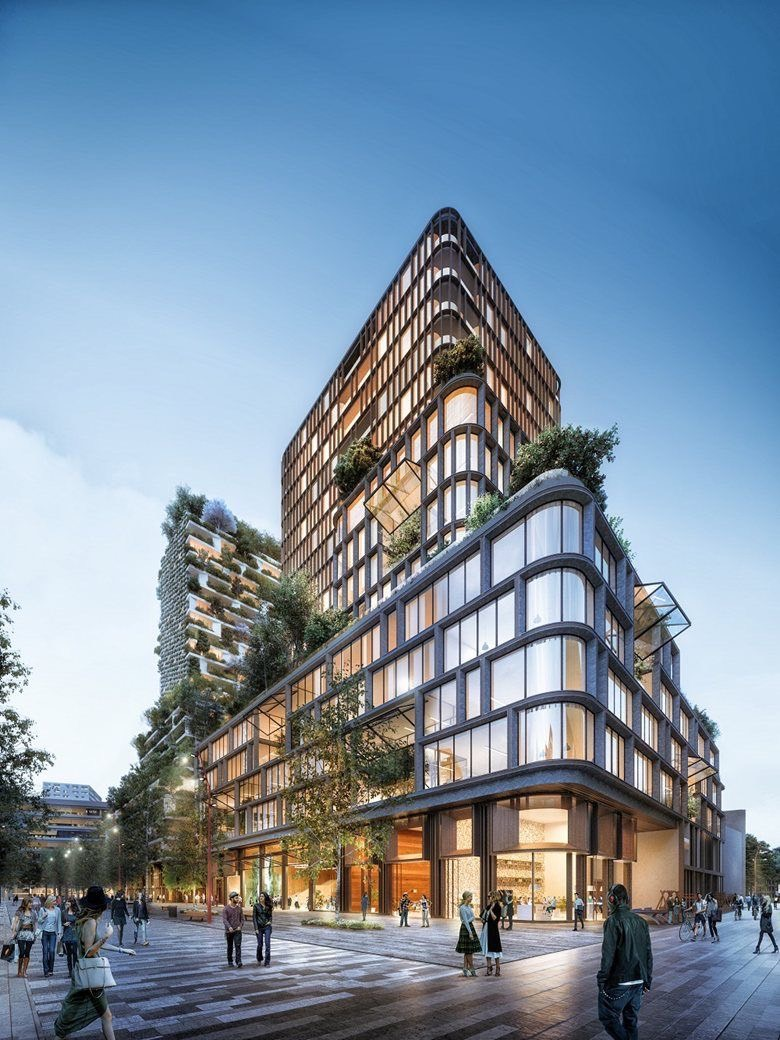
\includegraphics[scale=0.2]{hotel.jpg}
    \caption{ภาพโรงแรม}
    \label{fig:graph1}
\end{figure}

\hspace{1cm}โรงแรม หมายถึง สถานที่ประกอบการเชิงการค้าที่นักธุรกิจตั้งขึ้น เพื่อบริการผู้เดินทางในเรื่องของที่พักอาศัย อาหาร และบริการอื่น ๆ ที่เกี่ยวข้องกับการพักอาศัยและเดินทาง หรืออาคารที่มีห้องนอนหลายห้อง ติดต่อเรียงรายกันในอาคารหนึ่งหลังหรือหลายหลัง ซึ่งมีบริการต่าง ๆ เพื่อความสะดวกของผู้ที่มาพัก ซึ่งเรียกว่า "แขก" (guest)
\hspace{1cm}คำว่า hotel หรือ โรงแรมมีที่มาจากภาษาฝรั่งเศสซึ่งแปลว่า คฤหาสน์ โรงแรมแห่งแรกในยุโรปคือ Hotel de Hanri IV (โฮเทล เดอ อองรี กัต) เมื่อปี ค.ศ. 1788 โดยในสมัยก่อนใช้คำว่า hôtel และภายหลังได้เปลี่ยนตัวโอมาเป็นโอปกติในภาษาอังกฤษเป็น hotel เหมือนปัจจุบัน\cite{history}

\hspace{1cm}ลักษณะของการดำเนินการจัดการโรงแรมในอดีตกับปัจจุบัน ต้องมีความแตกต่างกันไม่มากก็น้อย เนื่องจากปัจจัยหลายอย่าง เช่น ขนาดของที่พักแรม สถานที่ตั้ง รวมไปถึงสิ่งอำนวยความสะดวกที่มีไว้ให้บริการ เป็นต้นซึ่งในอดีตการบริหารธุรกิจที่พักแรมโดยส่วนมากเจ้าของจะเป็นผู้ดูแลและบริหารงานเองทั้งหมด แต่ในปัจจุบันธุรกิจโรงแรมได้ขายตัวขึ้นอย่างต่อเนื่อง และมีโรงแรมขนาดใหญ่จำนวนมาก จึงจำเป็นต้องมีการระดมเงินทุนหรือการรวมหุ้นเพื่อสร้างสิ่งดึงดูดใจให้ลูกค้าเลือกที่จะใช้บริการและเกิดความประทับใจ ประกอบกับการเดินทางที่สะดวกสบายในปัจจุบันส่งผลให้มีการเดินทางระหว่างประเทศอย่างกว้างขวาง ดังนั้นรูปแบบการบริหารจำต้องเปลี่ยนแปลงเป็นระบบที่ได้มาตรฐานและมืออาชีพ  ซึ่งอุตสาหกรรมที่พักแรมนั้นมีความสำคัญอยู่หลายด้าน ดังนี้ 
\begin{enumerate}
    \item{ด้านเศรษฐกิจ} \par
    ความเติบโตของกิจการด้านที่พักแรมและการท่องเที่ยว ย่อมส่งผลให้เกิดรายได้และการจ้างงานภายในประเทศ ทำให้เกิดการกระจายรายได้แก่ประชาชนในท้องถิ่น เช่น การทำธุรกิจท่องเที่ยวหรือธุรกิจอื่นที่เกี่ยวเนื่อง นอกจากนี้ยังมีรายได้อื่นๆ ตามมา เช่น การบริการจัดนำเที่ยว การขนส่ง ของพื้นถิ่น ฯลฯ จึงส่งผลให้อาชีพการบริการในธุรกิจการท่องเที่ยวมีการขยายตัวมากขึ้น เพื่อตอบสนองต่อความต้องการของนักท่องเที่ยว โดยความสำคัญของธุรกิจโรงแรมด้านเศรษฐกิจคือ
        \begin{itemize}
            \item ทำให้เกิดการสร้างงานและอาชีพ
            \item นำรายได้สู่ประเทศและสร้างเงินหมุนเวียนในระบบเศรษฐกิจ
            \item เป็นแหล่งรับซื้อสินค้าและผลิตภัณฑ์จากอุตสาหกรรมอื่นๆ ที่เกี่ยวข้อง เช่น อาหารและเครื่องดื่ม ของที่ระลึก ผลิตภัณฑ์ท้องถิ่น ของประดับตกแต่ง เป็นต้น
            \item สนับสนุนกิจกรรมทางการท่องเที่ยวและส่งเสริมการลงทุนในภูมิภาค
        \end{itemize}
    \item{ด้านสังคม} \par
    สืบเนื่องจากการที่กิจการที่พักแรมส่งผลให้เกิดการกระจายรายได้และการจ้างงานนั้น ย่อมส่งผลให้คุณภาพชีวิตที่ดีขึ้น เพราะมีการกระจายรายได้ไปยังส่วนต่างๆ ในชุมชนที่มีแหล่งท่องเที่ยวหรือสถานที่สำคัญ และสมารถดึงดูดนักท่องเที่ยว ทำให้มีรายได้จากธุรกิจการท่องเที่ยว ลดปัญหาการว่างงาน และการอพยพแรงงานเข้าสู่เมืองใหญ่ ความสำคัญของธุรกิจที่พักแรมด้านสังคม คือ
        \begin{itemize}
            \item สามารถยกระดับมาตรฐานความเป็นอยู่ท้องถิ่นจากการมีรายได้เพิ่มมากขึ้น เช่น ระบบคมนาคมขนส่ง ความปลอดภัย ระบบสาธารณูปโภค เป็นต้น
            \item ลดปัญหาการว่างงานและชุมชนแออัด จากการอพยพแรงงานเข้าสู่เมืองใหญ่ อันจะเป็นผลที่ทำให้เกิดปัญหาสังคมตามมา
            \item เป็นแหล่งบันเทิงของชุมชนเพื่อการพักผ่อน
            \item เป็นแหล่งพบปะสังสรรค์และศูนย์รวมกิจกรรมทางสังคม เช่น การจัดโครงการต่างๆ การจัดประชุมสัมมนา งานสังสรรค์ \cite{his}
        \end{itemize}
\end{enumerate} 

\pagebreak

\section{วัตถุประสงค์}
\begin{itemize}
    \item{เพื่อสามารถประยุกต์ใช้เทคนิควิธีวิเคราะห์และออกแบบฐานข้อมูลและสร้างเว็บให้มีประสิทธิภาพได้}
    \item{เพื่อให้ความรู้ ความเข้าใจของระบบฐานข้อมูล}
    \item{เพื่อเพื่อตอบปัญหาตอบคำถามที่กำหนดขึ้นได้จริง}
\end{itemize}

\section{ประโยชน์ที่คาดว่าจะได้รับ}
\begin{itemize}
    \item{สามารถประยุกต์ใช้เทคนิควิธีวิเคราะห์และออกแบบฐานข้อมูลและสร้างเว็บให้มีประสิทธิภาพได้}
    \item{ได้ความรู้ ความเข้าใจของระบบฐานข้อมูล}
    \item{ตอบปัญหาตอบคำถามที่กำหนดขึ้นได้จริง}
\end{itemize}
 
\chapter{ความรู้ทั่วไป}

\section{การจัดแบ่งประเภทห้องพัก}
ห้องพักทางโรงแรมมีจำนวน 10 ประเภท ดังนี้ \par

\begin{table}[h!]
\centering
\begin{tabular}{|c|c|c|c|c|}
\hline
ประเภทที่ & ชื่อประเภทห้องพัก & ขนาดห้อง(ตร.ม) & จำนอนลูกค้าที่เข้าพักได้ & ราคาปกติ \\
\hline
1 & Deluxe Room & 30 & 2 & 2500 \\
2 & Superior Room & 35 & 3 & 3500 \\
3 & Family Suite & 50 & 4 & 4500 \\
4 & Executive Suite & 60 & 2 & 6000 \\
5 & Single Room & 20 & 1 & 1500 \\
6 & Double Room & 25 & 2 & 2000 \\
7 & Presidential Suite & 100 & 4 & 10000 \\
8 & Standard Room & 25 & 2 & 1800 \\
9 & Studio & 40 & 2 & 3000 \\
10 & Penthouse Suite & 120 & 4 & 12000 \\
\hline
\end{tabular}
\caption{ประเภทห้องพัก}
\label{table:1}
\end{table}

\section{ตัวอย่างห้องพัก}
\begin{figure}
    \centering
    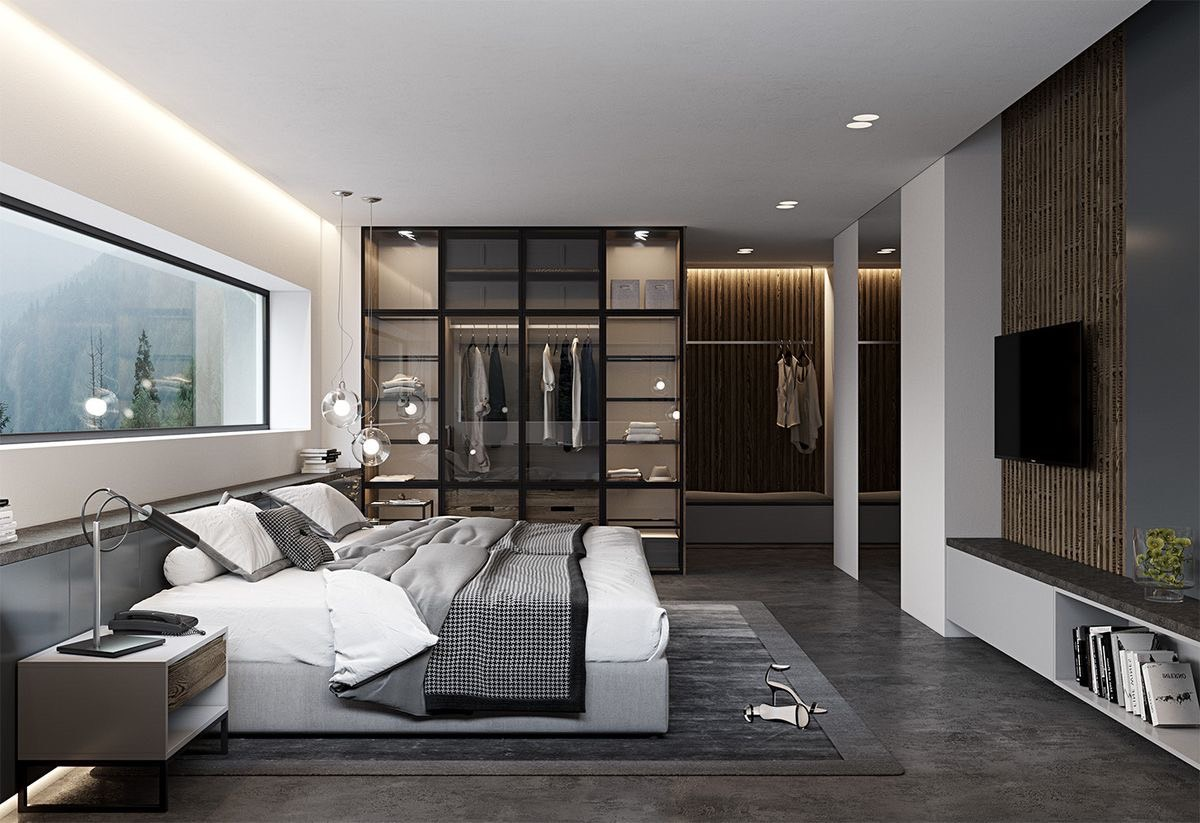
\includegraphics[scale=0.2]{Deluxe.jpg}
    \caption{ตัวอย่างห้อง Deluxe Room}
    \label{fig:graph2}
\end{figure}

\begin{figure}
    \centering
    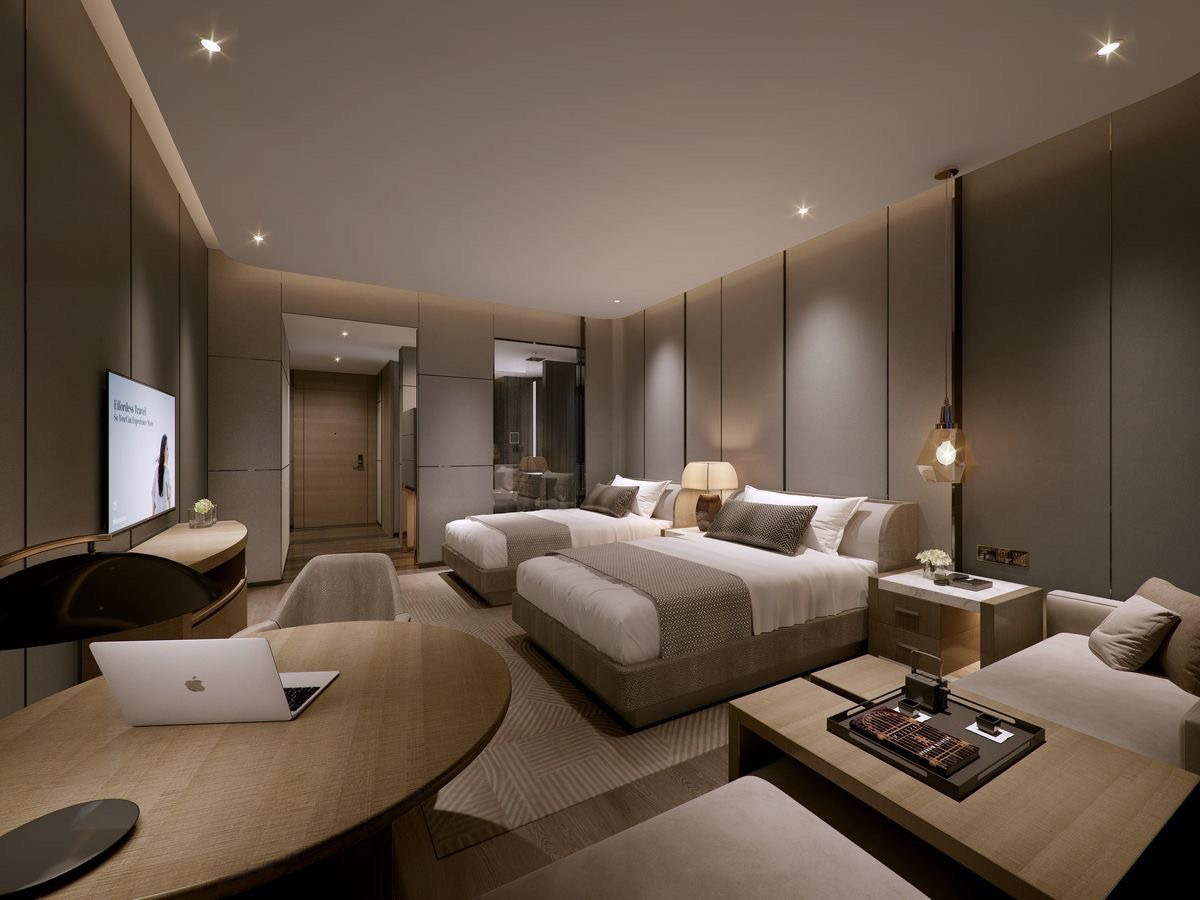
\includegraphics[scale=0.2]{Superior.jpg}
    \caption{ตัวอย่างห้อง Superior Room}
    \label{fig:graph3}
\end{figure}

\begin{figure}
    \centering
    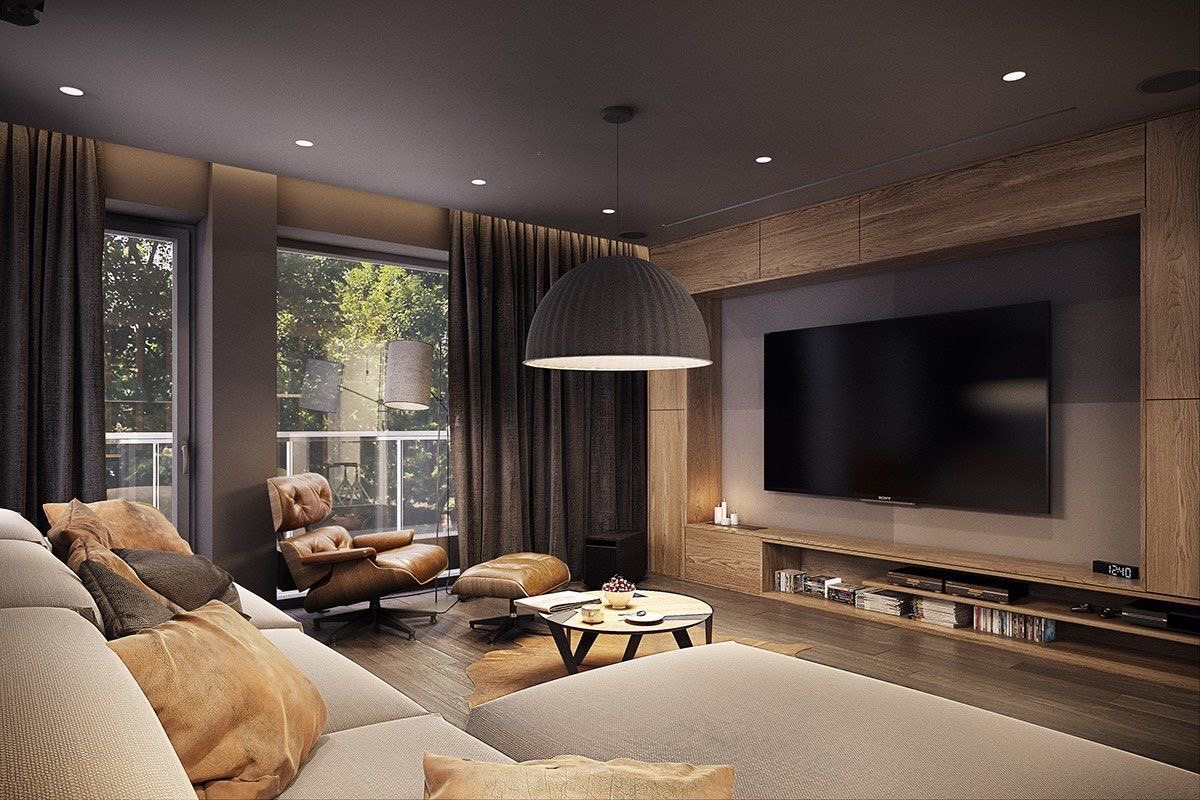
\includegraphics[scale=0.2]{Family.jpg}
    \caption{ตัวอย่างห้อง Family Suite}
    \label{fig:graph4}
\end{figure}

\begin{figure}
    \centering
    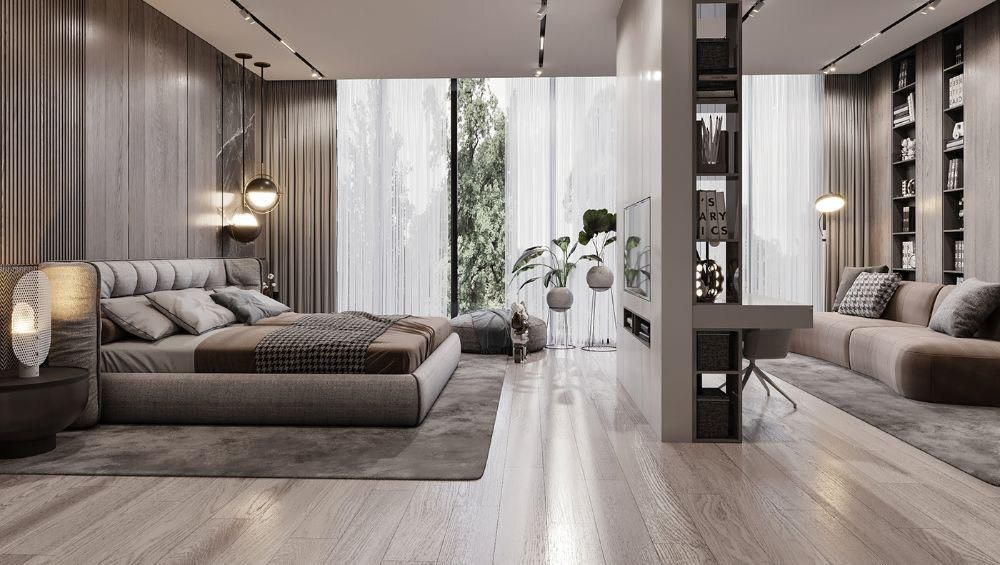
\includegraphics[scale=0.2]{Executive.jpg}
    \caption{ตัวอย่างห้อง Executive Suite}
    \label{fig:graph5}
\end{figure}

\begin{figure}
    \centering
    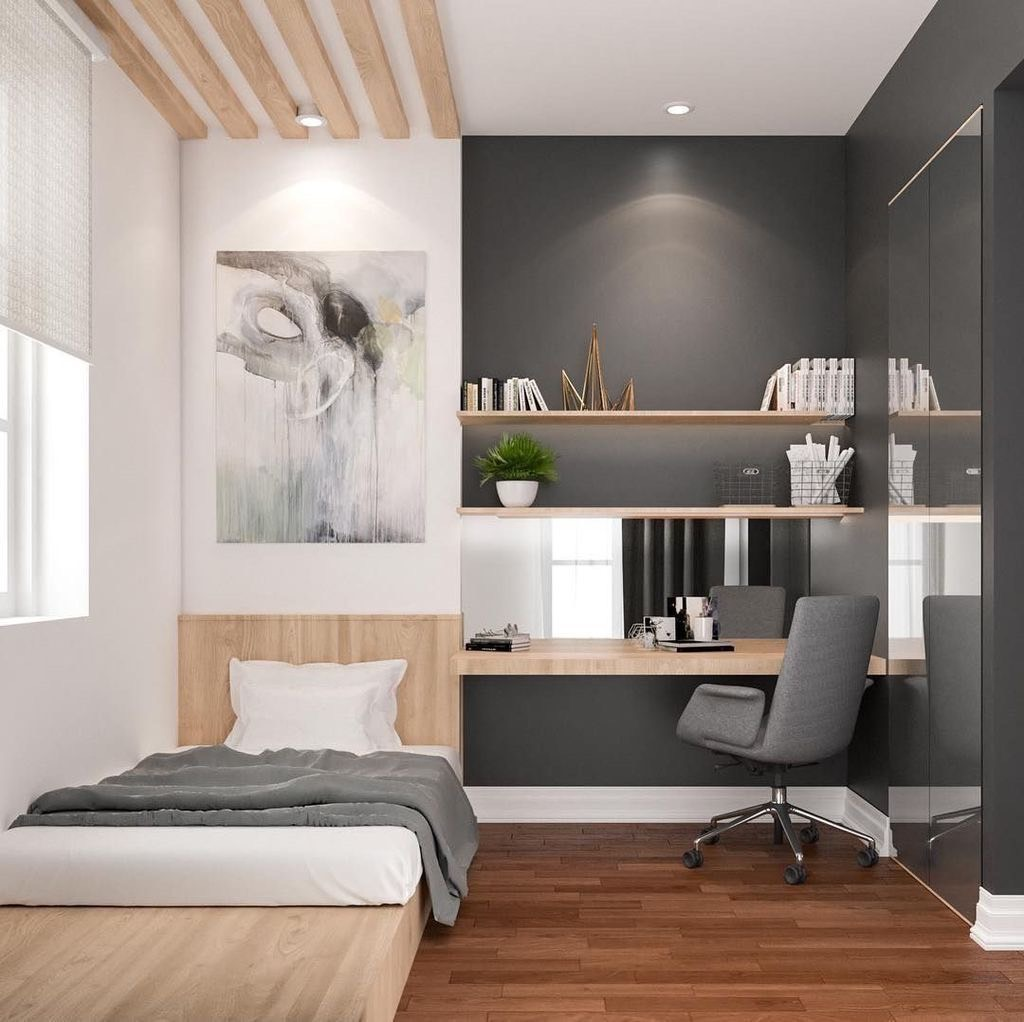
\includegraphics[scale=0.2]{Single.jpg}
    \caption{ตัวอย่างห้อง Single Room}
    \label{fig:graph6}
\end{figure}

\begin{figure}
    \centering
    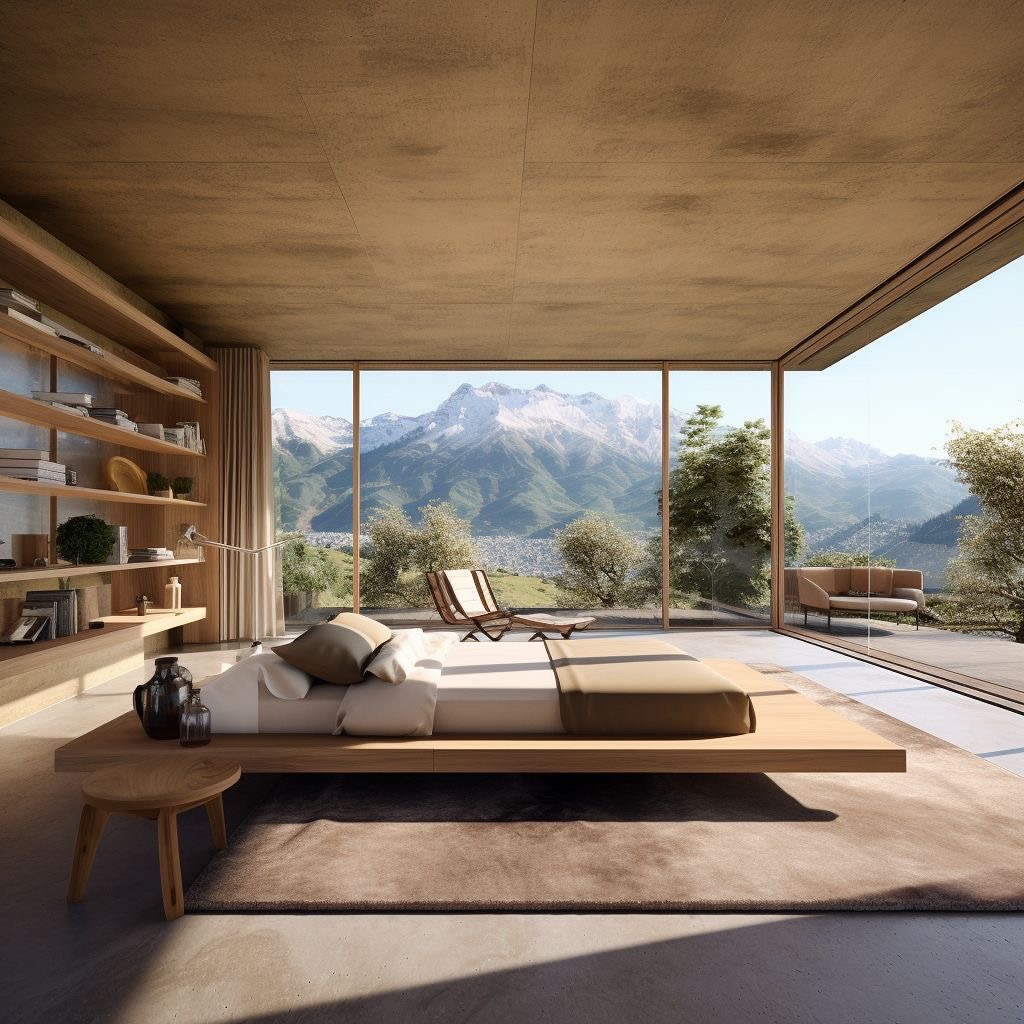
\includegraphics[scale=0.1]{Double.jpg}
    \caption{ตัวอย่างห้อง Double Room}
    \label{fig:graph7}
\end{figure}

\begin{figure}
    \centering
    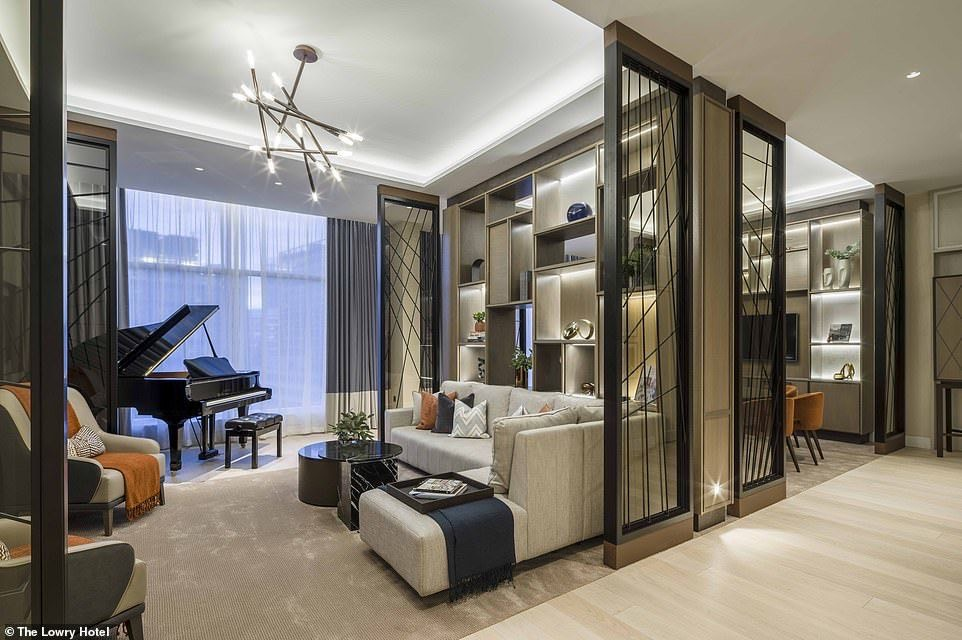
\includegraphics[scale=0.2]{Presidential.jpg}
    \caption{ตัวอย่างห้อง Presidential Suite}
    \label{fig:graph8}
\end{figure}

\begin{figure}
    \centering
    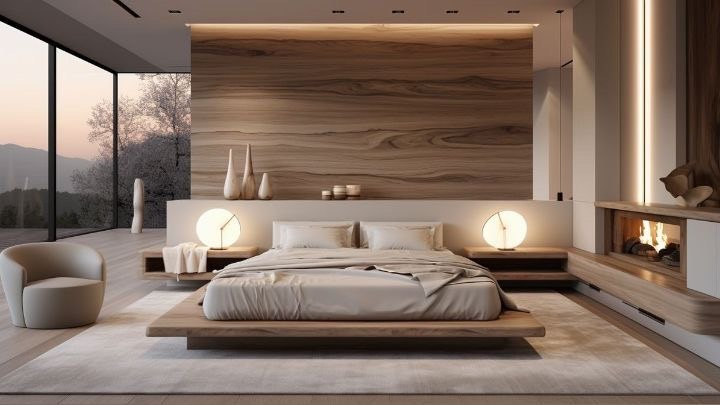
\includegraphics[scale=0.2]{Standard.jpg}
    \caption{ตัวอย่างห้อง Standard Room}
    \label{fig:graph9}
\end{figure}

\begin{figure}
    \centering
    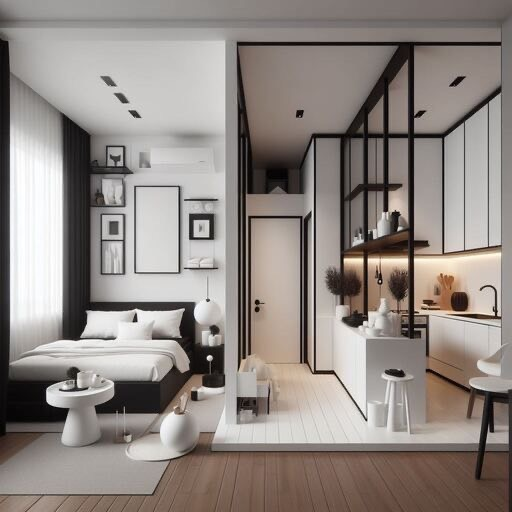
\includegraphics[scale=0.2]{Studio.jpg}
    \caption{ตัวอย่างห้อง Studio}
    \label{fig:graph10}
\end{figure}

\begin{figure}
    \centering
    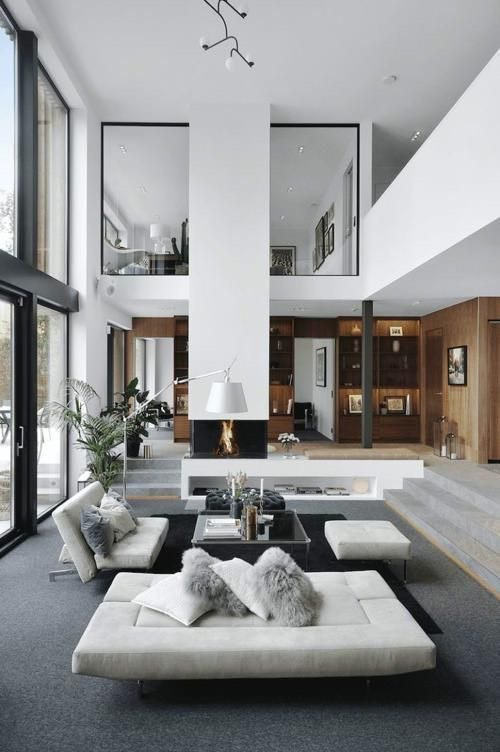
\includegraphics[scale=0.2]{Penthouse.jpg}
    \caption{ตัวอย่างห้อง Penthouse Suite}
    \label{fig:graph11}
\end{figure}

\pagebreak

\section{สิ่งอำนวยความสะดวกของห้องแต่ละประเภท}
\begin{table}[h!]
\centering
\begin{tabular}{|c|c|}
\hline
ชื่อประเภทห้องพัก & สิ่งอำนวยความสะดวก \\
\hline
Deluxe Room & อินเตอร์เน็ต,ทีวี,เครื่องปรับอากาศ,มินิบาร์  \\
Superior Room & อินเตอร์เน็ต,ทีวี,เครื่องปรับอากาศ,ระเบียง \\
Family Suite & อินเตอร์เน็ต,ทีวี,เครื่องปรับอากาศ,ห้องครัว, ห้องนั่งเล่น \\
Executive Suite & อินเตอร์เน็ต,ทีวี,เครื่องปรับอากาศ,มินิบาร์,โต๊ะทำงาน,สิทธิ์เข้าใช้เลานจ์ \\
Single Room & อินเตอร์เน็ต,ทีวี,เครื่องปรับอากาศ \\
Double Room & อินเตอร์เน็ต,ทีวี,เครื่องปรับอากาศ,มินิบาร์ \\
Presidential Suite & อินเตอร์เน็ต,ทีวี,เครื่องปรับอากาศ,มินิบาร์,สระว่ายน้ำส่วนตัว,ห้องครัว,ห้องรับประทานอาหาร \\
Standard Room & อินเตอร์เน็ต,ทีวี,เครื่องปรับอากาศ \\
Studio & อินเตอร์เน็ต,ทีวี,เครื่องปรับอากาศ,ครัวขนาดเล็ก,ระเบียง \\
Penthouse Suite & อินเตอร์เน็ต,ทีวี,เครื่องปรับอากาศ,มินิบาร์,ระเบียงส่วนตัว,อ่างจากุซซี่,ห้องรับประทานอาหาร \\
\hline
\end{tabular}
\caption{สิ่งอำนวยความสะดวกของห้องแต่ละประเภท}
\label{table:2}
\end{table}


\pagebreak

\section{ปัจจัยการตั้งราคาขายห้องพักโรงแรม-ที่พัก}
\subsection{ต้นทุน}
ต้นทุนในการบริหารโรงแรม ได้แก่ ต้นทุนค่าเช่าพื้นที่ ค่าสาธารณูปโภค ค่าจ้างพนักงาน ค่าการตลาด ผู้ประกอบการควรคำนวณต้นทุนทั้งหมดอย่างรอบคอบ เพื่อกำหนดราคาห้องพักให้เพียงพอต่อต้นทุนและสร้างกำไร
\subsection{กำไรที่ต้องการ}
ควรมี Minimum ของกำไรที่ต้องการ ต้องหากำไรในจุดที่ต่ำสุดที่รับได้ ให้เป็นแนวทางในการตั้งราคาขาย
\subsection{ความต้องการ}
โรงแรมที่พักควรศึกษาความต้องการห้องพักในบริเวณใกล้เคียง เพื่อกำหนดราคาห้องพักให้สอดคล้องกับความต้องการ หากอยู่ในพื้นที่ที่มีนักท่องเที่ยวมาเป็นจำนวนมาก ก็ปรับราคาห้องพักให้สูงขึ้นได้
\subsection{ปัจจัยด้านฤดูกาล}
ความต้องการห้องพักจะแตกต่างกันไปในแต่ละฤดูกาล ในช่วงที่มีความต้องการห้องพักสูง เช่น เทศกาลท่องเที่ยว ผู้ประกอบการอาจปรับราคาห้องพักให้สูงขึ้นได้
\subsection{ปัจจัยด้านสภาพเศรษฐกิจ}
ภาวะเศรษฐกิจโดยรวมมีผลต่อความต้องการห้องพักเช่นกัน ในช่วงที่เศรษฐกิจไม่ดี ผู้ประกอบการอาจปรับราคาห้องพักให้ลดลงได้
\subsection{กลุ่มลูกค้า}
คำนึงถึงโรงแรมที่พักว่าเป้าหมายเป็นกลุ่มลูกค้าระดับไหน มีกำลังซื้อมากน้อยเพียงใด 
\subsection{คู่แข่ง}
กำหนดราคาห้องพักให้สอดคล้องกับราคาห้องพักของโรงแรมคู่แข่งในบริเวณใกล้เคียง กลยุทธ์นี้มีข้อดีคือ ช่วยให้โรงแรมสามารถแข่งขันกับคู่แข่งได้ แต่อาจทำให้ผู้ประกอบการขาดรายได้หากราคาห้องพักของคู่แข่งต่ำกว่า จึงต้องกลับไปมองกำไรในจุดต่ำสุดที่รับได้ด้วย
\subsection{ตั้งราคาตามคุณค่าและความเป็นตัวตน}
กำหนดราคาห้องพักโดยมองจาก  การกำหนดระดับโรงแรม คอนเซ็ปต์ที่สร้างตัวตนของที่พักว่าจะวางอยู่ในระดับไหน รวมถึงพิจารณาจากคุณค่าที่ลูกค้าได้รับเมื่อมาเข้าพัก\cite{price}

\section{โรงแรมมีการเพิ่มราคาค่าห้องพักอย่างไร}
ปัจจัยมากมายที่จะมีผลต่อการกำหนดราคาของห้องพัก ดังนี้
\subsection{ปัจจัยเทศกาล}
ความต้องการห้องพักจะแตกต่างกันไปในแต่ละฤดูกาล ในช่วงที่มีความต้องการห้องพักสูง เช่น เทศกาลท่องเที่ยว ผู้ประกอบการอาจปรับราคาห้องพักให้สูงขึ้นได้ \par
โดยทางโรงแรมของเราการเพิ่มขึ้นของราคาในช่วงเทศกาล ดังนี้
\begin{itemize}
    \item{ช่วงเดือนมกราคม มีการบวกเพิ่มราคาห้องพักจากราคาเดิม 500บาท}
    \item{ช่วงเดือนกุมภาพันธ์ มีการบวกเพิ่มราคาห้องพักจากราคาเดิม 600บาท}
    \item{ช่วงเดือนมีนาคม มีการบวกเพิ่มราคาห้องพักจากราคาเดิม 550บาท}
    \item{ช่วงเดือนเมษายน มีการบวกเพิ่มราคาห้องพักจากราคาเดิม 620บาท}
    \item{ช่วงเดือนพฤศจิกายน มีการบวกเพิ่มราคาห้องพักจากราคาเดิม 720บาท}
    \item{ช่วงเดือนธันวาคม มีการบวกเพิ่มราคาห้องพักจากราคาเดิม 720บาท}
\end{itemize}


\chapter{ปัญหาและการแก้ปัญหาของระบบฐานข้อมูลที่กำหนด}

\begin{figure}[h!]
\centering
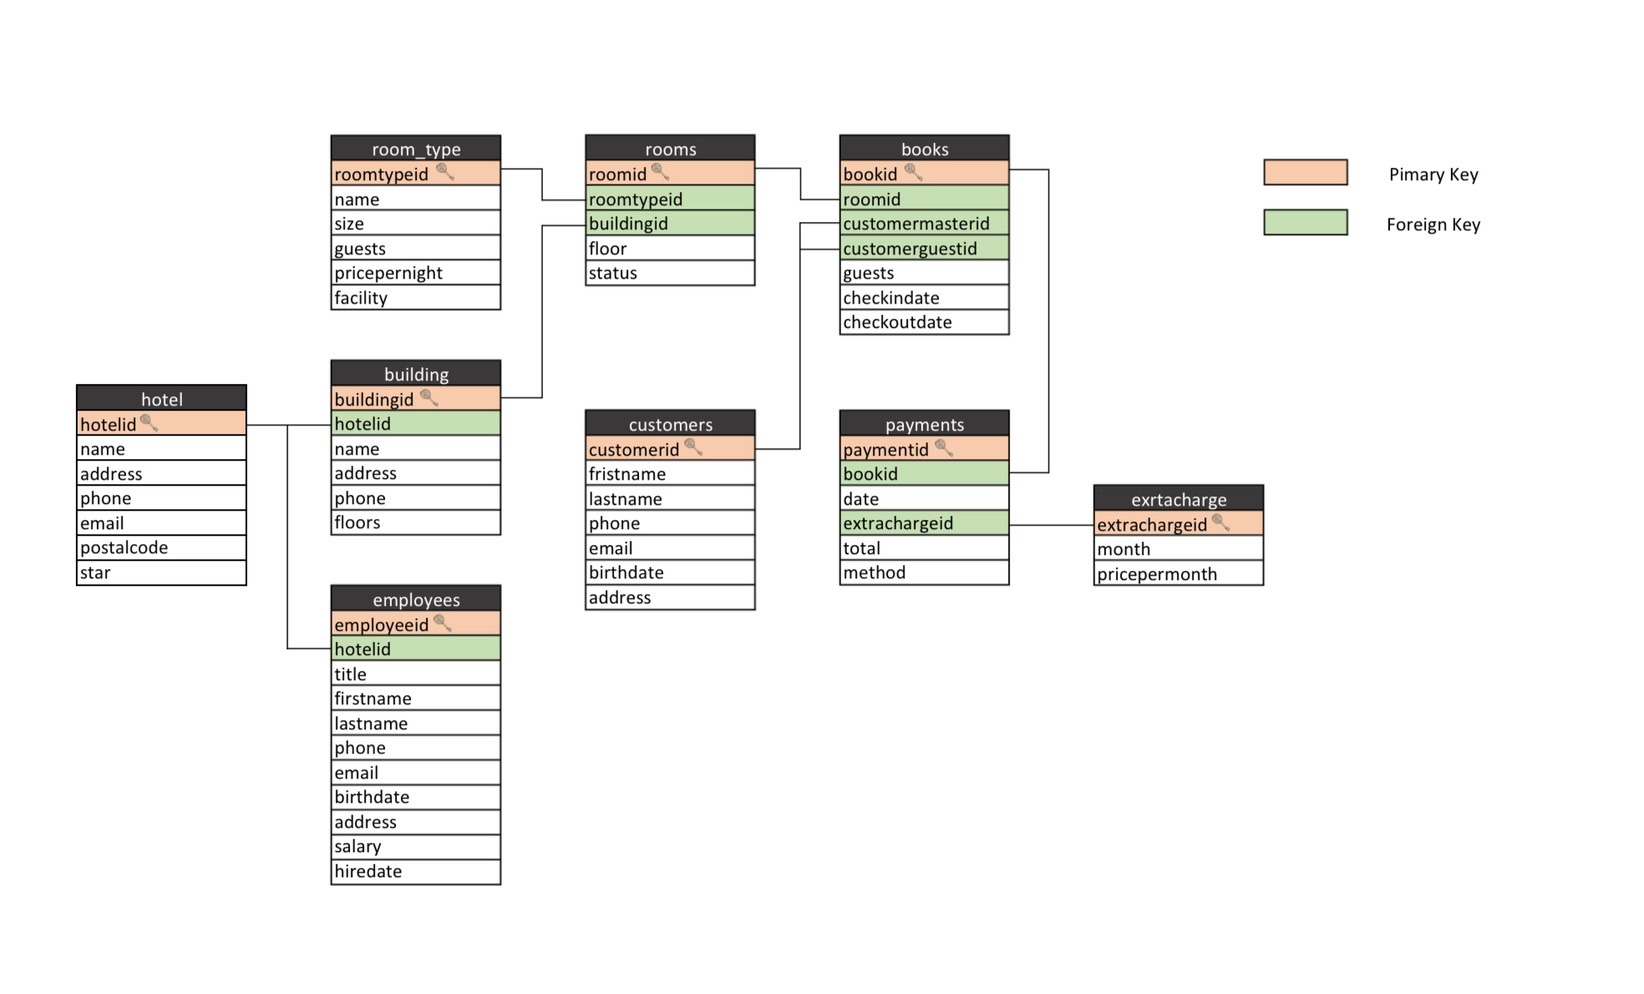
\includegraphics[scale=0.25]{diagram.jpg}
\caption{ตารางข้อมูล} 
\label{fig:graph12}
\end{figure} 

\pagebreak

\section{ปัญหาของระบบฐานข้อมูล การแก้ปัญหาและผลลัพธ์ มีดังนี้}
\subsection{ปัญหาที่1 ลูกค้าเข้าพักช่วงเดือนไหนมากที่สุด}
\subsection{โค้ดในการแก้ปัญหา}
\begin{verbatim}
SELECT 
 strftime('%m', check_in_date) AS month, 
 COUNT(*) AS total_bookings
FROM books
GROUP BY month
ORDER BY total_bookings DESC;
\end{verbatim}

\subsection{ผลลัพธ์}

\begin{figure}[h!]
\centering
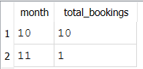
\includegraphics[scale=0.75]{month.png}
\caption{ผลลัพธ์ของโค้ด} 
\label{fig:graph13}
\end{figure} 

ดังนั้น ลูกค้าเข้าพักช่วง เดือนตุลาคม มากที่สุด

\pagebreak

\subsection{ปัญหาที่2 ห้องประเภทไหนที่ลูกค้าเข้าพักมากที่สุด}
\subsection{โค้ดในการแก้ปัญหา}
\begin{verbatim}
SELECT 
 rt.name AS room_type, 
 COUNT(b.book_id) AS total_bookings
FROM books b
JOIN rooms r ON b.room_id = r.room_id
JOIN room_type rt ON r.room_type_id = rt.room_type_id
GROUP BY rt.name
ORDER BY total_bookings DESC;
\end{verbatim}

\subsection{ผลลัพธ์}
\begin{figure}[h!]
\centering
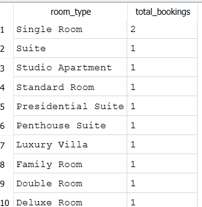
\includegraphics[scale=0.75]{room.png}
\caption{ผลลัพธ์ของโค้ด} 
\label{fig:graph14}
\end{figure} 

ดังนั้น ลูกค้าเข้าพักห้องประเภท Single Room มากที่สุด

\pagebreak

\subsection{ปัญหาที่3 จำนวนลูกค้าอยู่ในช่วงอายุใดมากที่สุด}
\subsection{โค้ดในการแก้ปัญหา}
\begin{verbatim}
SELECT 
 CASE 
  WHEN age BETWEEN 0 AND 4 THEN '0-4'
  WHEN age BETWEEN 5 AND 9 THEN '5-9'
  WHEN age BETWEEN 10 AND 14 THEN '10-14'
  WHEN age BETWEEN 15 AND 19 THEN '15-19'
  WHEN age BETWEEN 20 AND 24 THEN '20-24'
  WHEN age BETWEEN 25 AND 29 THEN '25-29'
  WHEN age BETWEEN 30 AND 34 THEN '30-34'
  WHEN age BETWEEN 35 AND 39 THEN '35-39'
  WHEN age BETWEEN 40 AND 44 THEN '40-44'
  WHEN age BETWEEN 45 AND 49 THEN '45-49'
  WHEN age >= 50 THEN '50+'
 END AS age_group,
 COUNT(*) AS customer_count
FROM (
 SELECT 
 strftime('%Y', 'now') - strftime('%Y', birth_date) AS age
 FROM customers
)
GROUP BY age_group
ORDER BY age_group;

\end{verbatim}

\subsection{ผลลัพธ์}

\begin{figure}[h!]
\centering
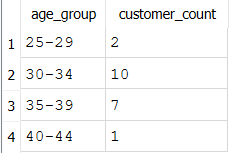
\includegraphics[scale=0.75]{age.png}
\caption{ผลลัพธ์ของโค้ด} 
\label{fig:graph15}
\end{figure} 

ดังนั้น ลูกค้าที่เข้าพักอยู่ในช่วงอายุ 30-34 ปี จำนวน 10 คน


\chapter{การดำเนินการในส่วนของเว็บไซต์(Website)}
\section{$โค้ดhotel_about.index$}

\begin{verbatim}
<!DOCTYPE html>
<html lang="en">
<head>
    <meta charset="UTF-8">
    <meta name="viewport" content="width=device-width, initial-scale=1.0">
    <title>SQLite Example</title>
    <link rel="stylesheet" href="hotel_style_server.css">
</head>
<body class="lob-bg">

    <header>
        <nav class="topnav">
            <a href="hotel_index.html">Home</a>
            <a href="hotel_books.html">Book Now</a>
            <a href="hotel_contact.html">Contact</a>
            <a href="https://www.google.co.th/maps/place/คณะวิทยาศาสตร์และเทคโนโลยี+มหาวิทยาลัยเทคโนโลยีราชมงคลธัญบุรี/@14.0387549,100.7267522,17.79z/data=!4m6!3m5!1s0x311d78a3cf303805:0x298cef6207b64026!8m2!3d14.0395596!4d100.7289406!16s%2Fg%2F12nvpzlcn?hl=th&entry=ttu&g_ep=EgoyMDI0MTAyOS4wIKXMDSoASAFQAw%3D%3D">Google Maps</a>
        </nav>
    </header>


    <nav class="navbar">
        <div>
            <h2>Select Table</h2>
            <select id="table-select">
                <option value="books">books</option>
                <option value="building">building</option>
                <option value="customers">customers</option>
                <option value="employees">employees</option>
                <option value="extracharge">extracharge</option>
                <option value="hotel">hotel</option>
                <option value="payments">payments</option>
                <option value="room_type">room_type</option>
                <option value="rooms">rooms</option>
            </select>
            <button type="button" id="table" onclick="fetchData()">Show All table</button>
        </div>
    
        <div>
            <h2>Filter Data</h2>
            <select id="column-select"></select>
            <input type="text" id="value-input" placeholder="Enter value">
            <button type="button" id="filter" onclick="fetchFilteredData()">Filter</button>
        </div>
    
        <div class="menu" id="menu">
            <h1>Question</h1>
            <form id="quary-Q">
                <button type="button" id="Q1" onclick="quaryQ1()">จำนวนลูกค้าต่อเดือน</button>
                <button type="button" id="Q2" onclick="quaryQ2()">จำนวนลูกค้าต่อประเภทห้องพัก</button>
                <button type="button" id="Q3" onclick="quaryQ3()">จำนวนลูกค้าตามช่วงอายุ</button>
            </form>
        </div>
    </nav>


    <div class="hide-data">
        <button type="button" id="hide-table" onclick="toggleTable()">Hide Table</button>
        <button type="button" id="hide-Q" onclick="toggleQ()">Hide Question</button>
    </div>

    <div class="show-data">
        <table id="data-table">
            <thead>
                <tr id="table-header"></tr>
            </thead>
            <tbody id="data-body"></tbody>
        </table>

        <table id="data-Q">
            <table id="list">
                <tbody class="Q">
        
                </tbody>
            </table>
        </table>
    </div>

    <script src="hotel_script.js"></script>
</body>

</html>
\end{verbatim}

\section{$โค้ดhotel_books.html$}
\begin{verbatim}
<!DOCTYPE html>
<html lang="en">
<head>
    <meta charset="UTF-8">
    <meta name="viewport" content="width=device-width, initial-scale=1.0">
    <title>The Hotel Sunshine</title>
    <link rel="stylesheet" href="hotel_style.css">
</head>
<body class="lob-bg">
    <header>
        <nav class="topnav">
            <a href="hotel_index.html">Home</a>
            <a href="hotel_contact.html">Contact</a>
            <a href="https://www.google.co.th/maps/place/คณะวิทยาศาสตร์และเทคโนโลยี+มหาวิทยาลัยเทคโนโลยีราชมงคลธัญบุรี/@14.0387549,100.7267522,17.79z/data=!4m6!3m5!1s0x311d78a3cf303805:0x298cef6207b64026!8m2!3d14.0395596!4d100.7289406!16s%2Fg%2F12nvpzlcn?hl=th&entry=ttu&g_ep=EgoyMDI0MTAyOS4wIKXMDSoASAFQAw%3D%3D">Google Maps</a>
        </nav>
    </header>

    <form action="/submit" method="post">
        <label for="firstname">First Name :</label>
        <input type="text" id="name" name="name" required>

        <label for="lastname">Last Name :</label>
        <input type="text" id="name" name="name" required>

        <label for="Phone">Phone number :</label>
        <input type="tel" id="Phone" name="Phone" required>

        <label for="birthday">Birthday :</label>
        <input type="date" id="birthday" name="birthday" required>

        <label for="email">Email :</label>
        <input type="email" id="email" name="email" required>
        
        <label for="address">Address :</label>
        <input type="text" id="address" name="address" required>

        <label for="guests">Guests :</label>
        <input type="number" id="guests" name="guests" minlength="0" required>

        <label for="building">Building :</label>
        <select name="building" id="building" required>
            <option value="Riverside Inn">Riverside Inn</option>
            <option value="Ocean View Tower">Ocean View Tower</option>
            <option value="Sunset Villas">Sunset Villas</option>
            <option value="Mountain Lodge">Mountain Lodge</option>
            <option value="Valley Resort">Valley Resort</option>
            <option value="Skyline Hotel">Skyline Hotel</option>
            <option value="Urban Suites">Urban Suites</option>
            <option value="Luxury Apartments">Luxury Apartments</option>
            <option value="Eco Lodge">Eco Lodge</option>
            <option value="City Center Tower">City Center Tower</option>
        </select>

        <label for="room_type">Room Type :</label>
        <select name="room_type" id="room_type" required>
            <option value="Single Room">Single Room</option>
            <option value="Standard Room">Standard Room</option>
            <option value="Double Room">Double Room</option>
            <option value="Deluxe Room">Deluxe Room</option>
            <option value="Family Room">Family Room</option>
            <option value="Suite Room">Suite Room</option>
            <option value="Studio Apartment">Studio Apartment</option>
            <option value="Luxury Villa">Luxury Villa</option>
            <option value="Penthouse Suite">Penthouse Suite</option>
            <option value="Presidential Suite">Presidential Suite</option>
        </select>

        <label for="room">Room :</label>
        <select name="room" id="room" required>
            <option value="2100">2100</option>
            <option value="2201">2201</option>
            <option value="2302">2302</option>
            <option value="2403">2403</option>
            <option value="2504">2504</option>
            <option value="2605">2605</option>
            <option value="2706">2706</option>
            <option value="2807">2807</option>
            <option value="2908">2908</option>
            <option value="2109">2109</option>
        </select>

        <label for="checkin">Check In :</label>
        <input type="date" id="checkin" name="checkin" required>
        <label for="time">Time :</label>
        <input type="time" id="time" name="time" required>

        <label for="checkout">Check Out :</label>
        <input type="date" id="checkout" name="checkout" required>
        <label for="time">Time :</label>
        <input type="time" id="time" name="time" required>
        
        <a href="#"><input type="submit" value="Submit"></a>
    </form>
</body>
</html>

\end{verbatim}

\section{$โค้ดhotel_contact.html$}
\begin{verbatim}
<!DOCTYPE html>
<html lang="en">
<head>
    <meta charset="UTF-8">
    <meta name="viewport" content="width=device-width, initial-scale=1.0">
    <title>The Hotel Sunshine</title>
    <link rel="stylesheet" href="hotel_style.css">
</head>
<body class="lob-bg">
    <header>
        <nav class="topnav">
            <nav class="topnav">
                <a href="hotel_index.html">Home</a>
                <a href="hotel_books.html">Book Now</a>
                <a href="https://www.google.co.th/maps/place/คณะวิทยาศาสตร์และเทคโนโลยี+มหาวิทยาลัยเทคโนโลยีราชมงคลธัญบุรี/@14.0387549,100.7267522,17.79z/data=!4m6!3m5!1s0x311d78a3cf303805:0x298cef6207b64026!8m2!3d14.0395596!4d100.7289406!16s%2Fg%2F12nvpzlcn?hl=th&entry=ttu&g_ep=EgoyMDI0MTAyOS4wIKXMDSoASAFQAw%3D%3D">Google Maps</a>
        </nav>
    </header>

    <div class="conbox" id="facebook"><a href="#">Facebook : The Hotel Sunshine</a></div>
    <div class="conbox" id="line"><a href="#">Line : @thehotelsunshine</a></div>
    <div class="conbox" id="instagram"><a href="#">Instagram : thehotelsunshine</a></div>
    <div class="conbox" id="tel"><a href="#">Tel: +66 (0)2 XXX XXXX-X | +66 (0)98 XXX XXXX</a></div>
    <div class="conbox" id="www"><a href="hotel_index.html">www.thehotelsunshine.com</a></div>
</body>
</html>
\end{verbatim}

\section{$โค้ดhotel_index.html$}
\begin{verbatim}
<!DOCTYPE html>
<html lang="en">
<head>
    <meta charset="UTF-8">
    <meta name="viewport" content="width=device-width, initial-scale=1.0">
    <title>The Hotel Sunshine</title>
    <link rel="stylesheet" href="hotel_style.css">
</head>
<body class="lob-bg">
    <header>
        <nav class="topnav">
            <nav class="topnav">
                <a href="hotel_books.html">Book Now</a>
                <a href="hotel_contact.html">Contact</a>
                <a href="https://www.google.co.th/maps/place/คณะวิทยาศาสตร์และเทคโนโลยี+มหาวิทยาลัยเทคโนโลยีราชมงคลธัญบุรี/@14.0387549,100.7267522,17.79z/data=!4m6!3m5!1s0x311d78a3cf303805:0x298cef6207b64026!8m2!3d14.0395596!4d100.7289406!16s%2Fg%2F12nvpzlcn?hl=th&entry=ttu&g_ep=EgoyMDI0MTAyOS4wIKXMDSoASAFQAw%3D%3D">Google Maps</a>
        </nav>
    </header>

    <div>
        <h1 class="mainhotel">
            <p class="welcome">WELCOME TO</p>
            <p class="namehotel">The Hotel Sunshine</p>
            <p class="resort">Resort & Spa</p>
        </h1>
    </div>

    <div id="shadow"></div>
    <div class="message">
        <br>
        <p><font size="10px" color="white">The Hotel Sunshine</font></p>
        <p>123 Beach Road, Pattaya &nbsp; 4 star</p>
            <hr><br>
            <p class="fontcen">
                "At our hotel, 'Crafting for Your Best Choice' 
                means we focus on making your stay great.
                We carefully plan every part of your visit, 
                from cozy rooms to friendly service, valuable,
                just for you. Choose us for a stay where comfort meets care,
                making it the best choice for your trip."
            </p>
            <p class="fontcen">
                โรงแรมของเรา 'สร้างสรรค์เพื่อเป็นทางเลือกที่ดีที่สุดของคุณ'
                เราใส่ใจทุกรายละเอียดเพื่อทำให้การพักของคุณยอดเยี่ยมที่สุด 
                เราวางแผนทุกส่วนของการเข้าพักของคุณอย่างรอบคอบ
                ตั้งแต่ห้องที่อบอุ่น สะอาด ไปจนถึงการบริการที่เป็นมิตร
                เราจะทำให้ The Hotel Sunshine เป็นทางเลือกที่ดีที่สุด
                สำหรับการเดินทางของคุณ     
            </p>
            <video loop width="320" height="240" autoplay muted>
                <source src="view_hotel.mp4" type="video/mp4">
                <source src="view_hotel.ogg" type="video/ogg">
            </video>
    </div>
      
    <div class="message">
        <br>
        <p><font size="7px" color="white">Question ?</font></p>
        <p>คำถามที่พบ</p>
            <hr><br>
            <p>"ลูกค้าพักห้องประเภทไหนมากที่สุด ?"</p>
            <p>"เดือนไหนที่มีลูกค้าเข้าพักมากที่สุด ?"</p>   
            <p>"ลูกค้าส่วนใหญ่ที่เข้าพักอายุประมาณเท่าไหร่ ?"</p>        
            <a id="about" href="hotel_about.html"><button>About</button></a>    
    </div>
    
    <div class="message-end">
        <h1 class="fontcen">Building</h1>
        <main class="buildnav">
            <div class="item">
                <a href="#"><div class="li">
                    <img src="river.jpg" alt="Riverside Inn">
                    <h2>Riverside Inn</h2>
                    <p>Zone A, 123 Royal St, Bangkok</p>
                    <p>
                        ที่พักตั้งอยู่ริมแม่น้ำ ให้บริการวิวทิวทัศน์ที่สวยงามของแม่น้ำและบรรยากาศที่เงียบสงบ 
                        เป็นสถานที่เหมาะสำหรับการพักผ่อนและทำกิจกรรมทางน้ำ 
                        เช่น พายเรือ ตกปลา หรือเดินเล่นริมแม่น้ำ
                    </p>
                </div></a>
                <a href="#"><div class="li">
                    <img src="ocean.jpg" alt="Ocean View Tower">
                    <h2>Ocean View Tower</h2>
                    <p>Zone A, 123 Royal St, Bangkok</p>
                    <p>
                        อาคารที่พักที่ตั้งอยู่ใกล้ชายทะเล ซึ่งมีห้องพักที่สามารถมองเห็นวิวทะเลได้
                        จากหน้าต่างหรือระเบียง โดยทั่วไปแล้ว อาคารเหล่านี้มักมีสิ่งอำนวยความสะดวกที่หลากหลาย 
                        เช่น สระว่ายน้ำ ร้านอาหาร และพื้นที่สำหรับกิจกรรมต่าง ๆ
                    </p>
                </div></a>
                <a href="#"><div class="li">
                    <img src="sunset.jpg" alt="Sunset Villas">
                    <h2>Sunset Villas</h2>
                    <p>Zone C, 123 Royal St, Bangkok</p>
                    <p>
                        รีสอร์ทหรือวิลล่า ตั้งอยู่ในทำเลที่สามารถชมวิวพระอาทิตย์ตกได้ ซึ่งจะมีบรรยากาศที่เงียบสงบและโรแมนติก 
                        โดยทั่วไปแล้ว วิลล่าประเภทนี้มักมีสิ่งอำนวยความสะดวกที่ครบครัน เช่น สระว่ายน้ำส่วนตัว, ครัว, 
                        และพื้นที่นั่งเล่นกลางแจ้ง เพื่อให้ผู้เข้าพักได้สัมผัสกับความสวยงามของธรรมชาติ     
                    </p>
                </div></a>
                <a href="#"><div class="li">
                    <img src="mountain.jpg" alt="Mountain Lodge">
                    <h2>Mountain Lodge</h2>
                    <p>Zone B, 123 Royal St, Bangkok</p>
                    <p>
                        ตั้งอยู่ใกล้ภูเขาหรือพื้นที่ธรรมชาติที่สูง มีบรรยากาศที่อบอุ่นและเป็นกันเอง 
                        ซึ่งเหมาะสำหรับการพักผ่อนและทำกิจกรรมกลางแจ้ง เช่น การเดินป่า สกี หรือสำรวจธรรมชาติ
                        ที่พักเหล่านี้มักมีสิ่งอำนวยความสะดวกที่ออกแบบมาเพื่อให้ผู้เข้าพักรู้สึกสบาย เช่น ห้องนอนที่สะดวกสบาย 
                        ห้องนั่งเล่นที่อบอุ่น หรือแม้แต่เตาผิง นอกจากนี้ ยังมีร้านอาหารหรือบาร์ที่ให้บริการอาหารและเครื่องดื่มท่ามกลางวิวภูเขาที่สวยงาม     
                    </p>
                    </div></a>
                <a href="#"><div class="li">
                    <img src="garden.jpg" alt="Valley Resort">
                    <h2>Valley Resort</h2>
                    <p>Zone C, 123 Royal St, Bangkok</p>
                    <p>
                        รีสอร์ทที่ตั้งอยู่ในหุบเขาหรือพื้นที่ธรรมชาติที่ล้อมรอบด้วยภูเขา 
                        ซึ่งมักจะมีบรรยากาศที่เงียบสงบและเป็นธรรมชาติ ให้บริการห้องพักที่สะดวกสบายและสิ่งอำนวยความสะดวกต่าง ๆ 
                        เช่น สระว่ายน้ำ สปา หรือกิจกรรมกลางแจ้ง เช่น การเดินชมสวน ขี่จักรยาน 
                        เหมาะสำหรับผู้ที่ต้องการหลีกหนีจากความวุ่นวายของเมืองและค้นหาความสงบในธรรมชาติ     
                    </p>
                    </div></a>
                <a href="#"><div class="li">
                    <img src="sky.jpg" alt="Skyline Hotel">
                    <h2>Skyline Hotel</h2>
                    <p>Zone C, 123 Royal St, Bangkok</p>
                    <p>
                       ตึกสูงมีวิวที่สวยงาม ตั้งอยู่ในพื้นที่ที่มองเห็นทิวทัศน์ของเมืองหรือภูมิทัศน์โดยรอบ 
                       มีสิ่งอำนวยความสะดวกที่ทันสมัย เช่น ห้องอาหารที่มีวิวสวย ฟิตเนส 
                       และบริการอื่น ๆ ที่ช่วยให้ผู้เข้าพักได้สัมผัสกับความสะดวกสบาย     
                    </p>
                    </div></a>
                <a href="#"><div class="li">
                    <img src="urban.jpg" alt="Urban Suites">
                    <h2>Urban Suites</h2>
                    <p>Zone A, 123 Royal St, Bangkok</p>
                    <p>
                        ที่พักประเภทอพาร์ตเมนต์หรือห้องสวีท มีการตกแต่งที่ทันสมัยและให้ความสะดวกสบายเหมือนอยู่บ้าน 
                        ซึ่งเหมาะสำหรับนักเดินทางระยะยาวหรือนักธุรกิจ 
                        ที่พักประเภทนี้มักมีสิ่งอำนวยความสะดวก 
                        เช่น ครัวขนาดเล็ก ห้องนั่งเล่น และพื้นที่ทำงาน 
                        รวมถึงบริการเพิ่มเติมอย่าง Wi-Fi ฟรี ฟิตเนส และพื้นที่สันทนาการ 
                        สะดวกต่อการเข้าถึงร้านค้า ร้านอาหาร และสถานที่ท่องเที่ยวต่าง ๆ     
                    </p>
                    </div></a>
                <a href="#"><div class="li">
                    <img src="luxury_build.jpg" alt="Luxury Apartments">
                    <h2>Luxury Apartments</h2>
                    <p>Zone A, 123 Royal St, Bangkok</p>
                    <p>
                        อพาร์ตเมนต์ที่มีการตกแต่งหรูหราและสิ่งอำนวยความสะดวกระดับสูง 
                        มักมีพื้นที่กว้างขวางและคุณภาพวัสดุที่ดีเยี่ยม 
                        ซึ่งเหมาะสำหรับผู้ที่ต้องการความสะดวกสบายและความหรูหราในการใช้ชีวิตประจำวัน     
                    </p>
                    </div></a>
                <a href="#"><div class="li">
                    <img src="eco.jpg" alt="Eco Lodge">
                    <h2>Eco Lodge</h2>
                    <p>Zone B, 123 Royal St, Bangkok</p>
                    <p>
                        ที่พักที่เน้นการใช้ทรัพยากรอย่างยั่งยืนและมีความรับผิดชอบต่อสิ่งแวดล้อม เน้นความธรรมชาติ
                        เพื่อให้ผู้เข้าพักได้สัมผัสกับธรรมชาติอย่างใกล้ชิด 
                        ใช้วัสดุธรรมชาติและเทคนิคการก่อสร้างที่เป็นมิตรกับสิ่งแวดล้อม
                        ใช้พลังงานจากแสงอาทิตย์ หรือน้ำฝนเพื่อสนับสนุนการดำเนินงาน
                        มีการจัดการขยะและการใช้ทรัพยากรน้ำอย่างประหยัด
                        มีโปรแกรมหรือกิจกรรมที่ส่งเสริมการรักษาสิ่งแวดล้อม เช่น การเดินป่า การดูนก หรือการปลูกต้นไม้           
                    </p>
                    </div></a>
                <a href="#"><div class="li">
                    <img src="city_center.jpg" alt="City Center Tower">     
                    <h2>City Center Tower</h2>
                    <p>Zone B, 123 Royal St, Bangkok</p>
                    <p>
                        อาคารที่พักที่ตั้งอยู่ใจกลาง มีการออกแบบที่ทันสมัยและให้บริการที่สะดวกสบายสำหรับผู้เข้าพัก
                        ห้องพักที่มองเห็นวิวทุกโซนของสถานที่แห่งนี้ มีสิ่งอำนวยความสะดวกที่ครบครัน
                        เช่น ฟิตเนส, สระว่ายน้ำ, ห้องประชุม และบริการอื่น ๆ 
                        ที่ตอบโจทย์นักธุรกิจและนักท่องเที่ยว            
                    </p>
                    </div></a>
            </div>
        </main>
    </div>

    <hr>

    <div class="message-end">
        <h1 class="fontcen">Rooms</h1>
        <main class="roomnav">
            <div class="item">

                <a href="#"><div class="li">
                    <img src="single.jpg" alt="Single Room">
                    <h2>Single Room</h2>
                        <p>ห้องเตียงเดี่ยว (Single Room) รองรับผู้เข้าพัก 1 คน มี
                            หนึ่งเตียงขนาด 3x6 ฟุต สามารถเพิ่มเตียงเสริมได้ 
                            เรียกว่า Extra bed ต้องจ่ายค่าธรรมเนียมเพิ่ม 
                            ขนาดห้องโดยทั่วไปอยู่ระหว่าง 37-45 ตารางเมตร
                        </p>
                </div></a>

                <a href="#"><div class="li">
                    <img src="standard.jpg" alt="Standard Room">
                    <h2>Standard Room</h2>
                        <p>
                            ห้องสแตนดาร์ด (Standard Room) 
                            เป็นประเภทของห้องพักในโรงแรมที่มีขนาดกะทัดรัดที่สุด 
                            โดยห้องประเภทนี้จะมีสิ่งอำนวยความสะดวกพื้นฐานที่จำเป็น 
                            เช่น เตียงนอน ห้องน้ำ ทีวี และเครื่องปรับอากาศ 
                            เหมาะสำหรับผู้เข้าพักที่เดินทางคนเดียวหรือมาเป็นคู่ 
                            อีกทั้งยังสะดวกต่อการเข้าพักเพียงไม่กี่วันและต้องการห้องพักในราคาประหยัด 
                        </p>
                </div></a>

                <a href="#"><div class="li">
                    <img src="double.jpg" alt="Double Room">     
                    <h2>Double Room</h2>
                        <p>
                            ห้องคู่ (Double Room) คือมีสิ่งอำนวยความสะดวกเพิ่มขึ้น เช่น โซฟา และโต๊ะทำงาน 
                            ซึ่งเหมาะสำหรับผู้เข้าพักที่เดินทางมาทำงาน หรือพักผ่อน ไม่ว่าจะเข้าพักคนเดียว หรือเป็นคู่ 
                            อาจจะจัดเป็นเตียง Twin 2 เตียง หรือ เตียง Double(7 ฟุต) แค่เตียงเดียวก็ได้
                            เป็นห้องพักที่มีขนาดกว้างกว่าห้องสแตนดาร์ดเล็กน้อย โดยห้องประเภทนี้เหมาะสำหรับผู้ที่
                            ต้องการความสะดวกสบายมากขึ้นในการพักผ่อนเมื่อเทียบกับห้องแบบสแตนดาร์ด 
                            และยังต้องการพื้นที่ในการนั่งทำงานอย่างเหมาะสมด้วย
                        </p>
                </div></a>

                <a href="#"><div class="li">
                    <img src="deluxe.jpg" alt="Deluxe Room">
                    <h2>Deluxe Room</h2>
                        <p>
                            ห้องดีลักซ์ (Deluxe Room) 
                            เป็นห้องพักที่มีขนาดกว้างและหรูหรากว่าห้องซูพีเรีย 
                            โดยจะมีสิ่งอำนวยความสะดวกครบครันมากกว่า 
                            เช่น เตียงนอนขนาดใหญ่ โซฟา โต๊ะทำงาน ตู้เย็น มินิบาร์ โทรทัศน์จอใหญ่ 
                            และอ่างอาบน้ำเป็นต้น เหมาะสำหรับผู้เข้าพักที่ต้องการที่พักที่หรูหราและสะดวกสบาย 
                            สามารถเข้าพักคนเดียว เป็นคู่ หรือครอบครัวขนาดเล็กก็ได้
                        </p>
                </div></a>

                <a href="#"><div class="li">
                    <img src="family.jpg" alt="Family Room">
                    <h2>Family Room</h2>
                        <p>
                            ห้องครอบครัว (Family Room) เป็นห้องสำหรับครอบครัว 
                            โดยทั่วไปสามารถรองรับได้ประมาณ 4 คน 
                            จะประกอบไปด้วยเตียงขนาดใหญ่สำหรับนอน 2 คน 
                            และมีเตียงเดี่ยวอีก 2 เตียง แต่ถ้าหากเป็นครอบครัวใหญ่ที่มี ปู่-ยา ตา-ยาย มาด้วย 
                            ก็จะมีห้องพักแบบ Grand Family Suite ซึ่งจะมีเตียงขนาดใหญ่เพิ่มขึ้นมาอีก 1 เตียง
                        </p>
                </div></a>

                <a href="#"><div class="li">
                    <img src="suite.jpg" alt="Suite Room">
                    <h2>Suite Room</h2>
                        <p>
                            ห้องสวีท (Suite room) ห้องสวีทจะมีการแบ่งสัดส่วนชัดเจน 
                            และมักมีห้องนั่งเล่นแยกต่างหาก  ซึ่งมาพร้อมกับเฟอร์นิเจอร์และสิ่งอำนวยความสะดวกมากมาย 
                            เช่น เตียงนอนขนาดใหญ่ โซฟา โต๊ะทำงาน ตู้เย็น มินิบาร์ ห้องเตรียมอาหาร 
                            ห้องรับประทานอาหาร ห้องน้ำขนาดใหญ่พร้อมอ่างอาบน้ำ เป็นต้น 
                            เหมาะสำหรับผู้เข้าพักที่เดินทางมากับคู่รัก 
                            หรือเป็นครอบครัวที่ต้องการห้องพักที่หรูหราและสะดวกสบายเป็นพิเศษ
                        </p>
                </div></a>

                <a href="#"><div class="li">
                    <img src="studio.jpg" alt="Studio Apartment">     
                    <h2>Studio Apartment</h2>
                        <p>
                            ห้องพักแบบสตูดิโอ (Studio Room) คือ ห้องพักที่ลักษณะเหมือนห้องพักในคอนโด 
                            มีการแบ่งสัดส่วนของห้องชัดเจน แยกห้องนั่งเล่นออกจากห้องนอน 
                            อาจมีบริเวณครัวเล็ก ๆ ที่สามารถประกอบอาหารภายในห้องพักได้
                        </p>
                </div></a>

                <a href="#"><div class="li">
                    <img src="luxury.jpg" alt="Luxury Villa">
                    <h2>Luxury Villa</h2>
                        <p>
                            ลักซ์ชัวรี่ วิลล่า(Luxury Villa) คือห้องพักที่มีลักษณะเป็นบ้านพักส่วนตัว 
                            มีหลายห้องนอน บริเวณบ้านพักมีสวน มีลานจอดรถ 
                            หรือบางครั้งอาจจะมีสระว่ายน้ำส่วนตัวด้วย เรียกว่า Pool Villa 
                            และภายใน วิลล่า ก็ห้องรับแขก ห้องนอนมากกว่า 1 ห้อง 
                            มีห้องครัวให้ทำอาหารรับประทานได้ โดยห้องประเภทนี้ 
                            เหมาะกับครอบครัวกลุ่มใหญ่นอนได้หลาย ๆ คน ผู้สูงอายุ คู่รัก และ ท่านลูกค้าที่นั่งวีลแชร์
                        </p>
                </div></a>
                
                <a href="#"><div class="li">
                    <img src="penthouse.jpg" alt="Penthouse Suite">
                    <h2>Penthouse Suite</h2>
                        <p>
                            ห้องเพนท์เฮ้าส์สวีท (Penthouse Suite) 
                            คือห้องพักที่อยู่ในชั้นสูงสุดของอาคาร เช่น โรงแรมหรือคอนโดมิเนียม 
                            ซึ่งมักมีพื้นที่กว้างขวางและการตกแต่งที่หรูหรา 
                            รวมถึงวิวที่สวยงามจากหน้าต่างหรือระเบียง 
                            ห้องนี้มักมีสิ่งอำนวยความสะดวกที่เหนือกว่าห้องพักทั่วไป 
                            เช่น ห้องนอนหลายห้อง ห้องนั่งเล่นขนาดใหญ่ อ่างจากุซซี่ 
                            หรือแม้กระทั่งสระว่ายน้ำส่วนตัว เป็นต้น 
                            ทำให้เป็นตัวเลือกที่นิยมสำหรับผู้ที่ต้องการความสะดวกสบายและความเป็นส่วนตัว
                            ในระหว่างการเข้าพัก
                        </p>
                </div></a>
                
                <a href="#"><div class="li">
                    <img src="presidential.jpg" alt="Presidential Suite">
                    <h2>Presidential Suite</h2>
                        <p>
                            ห้องเพรซซิเดนเชิลสวีท (Presidential Suite) คือห้องพักระดับหรูที่สุด วิวดีที่สุด
                            ซึ่งออกแบบมาให้มีความสะดวกสบายและหรูหราเป็นพิเศษ โดดเด่นด้วยเฉลียงที่สวยงาม และมีพื้นที่กว้างขวาง ห้องมีสองชั้น
                            ห้องนี้มักจะมีพื้นที่กว้างขวางพร้อมกับสิ่งอำนวยความสะดวกที่ครบครัน 
                            เช่น ชั้นหนึ่งมีสองห้องนอน และชั้นสองมีสามห้องนอนขนาดใหญ่ 
                            มีห้องรับประทานอาหารขนาดใหญ่ ห้องนั่งเล่น 
                            แบ่งเป็นสัดส่วน รวมถึงห้องน้ำที่หรูหรา ห้องน้ำแขก และห้องทำงาน
                            บางแห่งอาจมีบริการพิเศษ เช่น เชฟส่วนตัว หรือบริการผู้ช่วยส่วนตัว   
                            และมักจะมีวิวที่สวยงามจากหน้าต่างหรือระเบียงที่กว้างขวาง 
                            เหมาะสำหรับแขกที่ต้องการความเป็นส่วนตัวและความสะดวกสบายสูงสุด
                        </p>
                </div></a>
                
            </div>
        </main>
    </div>
 

    <script src="hotel_script.js"></script>
</body>
</html>
\end{verbatim}

\section{$โค้ดhotel_script.js$}
\begin{verbatim}
let currentTable = '';
let show = true;
let showQ = true;

async function fetchData() {
    const tableName = document.getElementById('table-select').value;
    currentTable = tableName;
    fetch(`/table/${tableName}`)
        .then(response => {
            if (!response.ok) {
                throw new Error('Network response was not ok');
            }
            return response.json();
        })
        .then(data => {
            const tableHeader = document.getElementById('table-header');
            const dataBody = document.getElementById('data-body');
            dataBody.innerHTML = '';
            tableHeader.innerHTML = '';
            populateColumnSelect(data);

            if (data.length === 0) {
                dataBody.innerHTML = '<tr><td colspan="100%">No data found</td></tr>';
                return;
            }

            const columns = Object.keys(data[0]);
            columns.forEach(col => {
                const th = document.createElement('th');
                th.textContent = col;
                tableHeader.appendChild(th);
            });

            data.forEach(item => {
                const row = document.createElement('tr');
                columns.forEach(col => {
                    const td = document.createElement('td');
                    td.textContent = item[col];
                    row.appendChild(td);
                });
                dataBody.appendChild(row);
            });
        })
        .catch(error => console.error('Error fetching data:', error));
}

function populateColumnSelect(data) {
    const columnSelect = document.getElementById('column-select');
    columnSelect.innerHTML = '';
    if (data.length > 0) {
        const columns = Object.keys(data[0]);
        columns.forEach(col => {
            const option = document.createElement('option');
            option.value = col;
            option.textContent = col;
            columnSelect.appendChild(option);
        });
    }
}

function fetchFilteredData() {
    const tableName = currentTable;
    const columnName = document.getElementById('column-select').value;
    const value = document.getElementById('value-input').value;

    fetch(`/table/${tableName}?column=${columnName}&value=${encodeURIComponent(value)}`)
        .then(response => {
            if (!response.ok) {
                throw new Error('Network response was not ok');
            }
            return response.json();
        })
        .then(data => {
            const tableHeader = document.getElementById('table-header');
            const dataBody = document.getElementById('data-body');
            dataBody.innerHTML = '';
            tableHeader.innerHTML = '';

            if (data.length === 0) {
                dataBody.innerHTML = '<tr><td colspan="100%">No data found</td></tr>';
            }

            const columns = Object.keys(data[0]);
            columns.forEach(col => {
                const th = document.createElement('th');
                th.textContent = col; 
                tableHeader.appendChild(th);
            });

            data.forEach(item => {
                const row = document.createElement('tr');
                columns.forEach(col => {
                    const td = document.createElement('td');
                    td.textContent = item[col];
                    row.appendChild(td);
                });
                dataBody.appendChild(row);
            });
        })
        .catch(error => console.error('Error fetching data:', error));
}

function toggleTable() {
    const dataTable = document.getElementById('data-table');
    show = !show;

    if (show) {
        dataTable.style.display = 'table'; 
        document.getElementById('hide-table').textContent = 'Hide Table';
    } else {
        dataTable.style.display = 'none';
        document.getElementById('hide-table').textContent = 'Show Table'; 
    }
}

document.getElementById('table').addEventListener('click', fetchData);

async function quaryQ1() {
    let response = await fetch('/queryQ1');
    let users = await response.json();
    let userList = document.getElementById('list').getElementsByTagName('tbody')[0];
    userList.innerHTML = '<tr><td>month</td> <td>total_bookings</td> </tr>'; 
    users.forEach(user => {
        userList.innerHTML +=                 
            `<tr> 
                <td>${user.month}</td> 
                <td>${user.total_bookings}</td> 
            </tr>`;
    });
}

async function quaryQ2() {
    let response = await fetch('/queryQ2');
    let users = await response.json();
    let userList = document.getElementById('list').getElementsByTagName('tbody')[0];
    userList.innerHTML = '<tr><td>room_type</td> <td>total_bookings</td> </tr>'; 
    users.forEach(user => {
        userList.innerHTML +=                 
            `<tr> 
                <td>${user.room_type}</td> 
                <td>${user.total_bookings}</td> 
            </tr>`;
    });
}

async function quaryQ3() {
    let response = await fetch('/queryQ3');
    let users = await response.json();
    let userList = document.getElementById('list').getElementsByTagName('tbody')[0];
    userList.innerHTML = '<tr><td>age_group</td> <td>customer_count</td> </tr>'; 
    users.forEach(user => {
        userList.innerHTML +=                 
            `<tr> 
                <td>${user.age_group}</td> 
                <td>${user.customer_count}</td> 
            </tr>`;
    });
}

function toggleQ() {
    const dataTable = document.getElementById('list');
    showQ = !showQ;

    if (showQ) {
        dataTable.style.display = 'table'; 
        document.getElementById('hide-Q').textContent = 'Hide Question';
    } else {
        dataTable.style.display = 'none';
        document.getElementById('hide-Q').textContent = 'Show Question'; 
    }
}

document.getElementById('Q1').addEventListener('click', quaryQ1);
document.getElementById('Q2').addEventListener('click', quaryQ2);
document.getElementById('Q3').addEventListener('click', quaryQ3);
\end{verbatim}

\section{$โค้ดhotel_server.js$}
\begin{verbatim}
const express = require('express');
const bodyParser = require('body-parser');
const sqlite3 = require('sqlite3').verbose();
const path = require('path');

const app = express();
const port = 3000;

app.use(bodyParser.json());
app.use(bodyParser.urlencoded({ extended: true }));
app.use(express.static(path.join(__dirname)));

app.listen(port, () => {
    console.log(`Server running on http://localhost:${port}`);
});

const db = new sqlite3.Database('./hotel.db');

const allowedTables = ['books', 'building', 'customers', 'employees', 'extracharge', 'hotel', 'payments', 'room_type', 'rooms'];

app.get('/table/:table_name', (req, res) => {
    const tableName = req.params.table_name;

    if (!allowedTables.includes(tableName)) {
        return res.status(400).json({ error: 'Invalid table name' });
    }

    const column = req.query.column;
    const value = req.query.value;

    let query = `SELECT * FROM ${tableName}`;
    const params = [];

    if (column && value) {
        query += ` WHERE ${column} = ?`;
        params.push(value);
    }

    db.all(query, params, (err, rows) => {
        if (err) {
            return res.status(500).json({ error: err.message });
        }
        res.json(rows);
    });
});

app.get('/queryQ1', (req, res) => {
    const queryQ1 = 
        `SELECT 
            strftime('%m', check_in_date) AS month, 
            COUNT(*) AS total_bookings
        FROM 
            books
        GROUP BY 
            month
        ORDER BY 
            total_bookings DESC`;
    db.all(queryQ1, (err, rows) => {
        if (err) {
            res.status(500).json({ error: err.message });
            return;
        }
        res.json(rows);
    });
});

app.get('/queryQ2', (req, res) => {
    const queryQ2 = 
       `SELECT 
            rt.name AS room_type, 
            COUNT(b.book_id) AS total_bookings
        FROM 
            books b
        JOIN 
            rooms r ON b.room_id = r.room_id
        JOIN 
            room_type rt ON r.room_type_id = rt.room_type_id
        GROUP BY 
            rt.name
        ORDER BY 
            total_bookings DESC`;
    db.all(queryQ2, (err, rows) => {
        if (err) {
            res.status(500).json({ error: err.message });
            return;
        }
        res.json(rows);
    });
});

app.get('/queryQ3', (req, res) => {
    const queryQ3 = 
       `SELECT 
            CASE 
                WHEN age BETWEEN 0 AND 4 THEN '0-4'
                WHEN age BETWEEN 5 AND 9 THEN '5-9'
                WHEN age BETWEEN 10 AND 14 THEN '10-14'
                WHEN age BETWEEN 15 AND 19 THEN '15-19'
                WHEN age BETWEEN 20 AND 24 THEN '20-24'
                WHEN age BETWEEN 25 AND 29 THEN '25-29'
                WHEN age BETWEEN 30 AND 34 THEN '30-34'
                WHEN age BETWEEN 35 AND 39 THEN '35-39'
                WHEN age BETWEEN 40 AND 44 THEN '40-44'
                WHEN age BETWEEN 45 AND 49 THEN '45-49'
                WHEN age >= 50 THEN '50+'
            END AS age_group,
            COUNT(*) AS customer_count
        FROM (
            SELECT 
                strftime('%Y', 'now') - strftime('%Y', birth_date) AS age
            FROM 
                customers
        )
        GROUP BY 
            age_group
        ORDER BY 
            age_group`;
    db.all(queryQ3, (err, rows) => {
        if (err) {
            res.status(500).json({ error: err.message });
            return;
        }
        res.json(rows);
    });
});

app.get('/', (req, res) => {
    res.sendFile(path.join(__dirname, 'hotel_about.html'));
});
\end{verbatim}

\section{$โค้ดhotel_style.css$}
\begin{verbatim}
body {
    margin: 0;
    font-family: Arial, Helvetica, sans-serif;
    box-sizing: border-box;
}

.lob-bg {
    background: url(lob.png) no-repeat center fixed; 
    background-size: cover;
}


header {
    position: sticky;
    top: 0;
}


.topnav {
    display: flex;
    font-size: 20px;
    text-align: center;
    justify-content: flex-end;
    color: white;
    overflow: hidden;
}

  
.topnav a {
    float: left;
    display: block;
    color: white;
    text-align: center;
    padding: 14px 10px;
    text-decoration: none;
}
  
.topnav a:hover {
    background-color: white;
    color: black;
    transition: background-color 0.3s;
  }
  
#shadow{
    background-color: rgba(0, 0, 0, 0.699);
    padding: 300px 100px;
    width: 20%;
    height: 100%;
    z-index: 1;
    top: 0;
    left: 0;
    overflow-x: hidden;
}

.mainhotel{
    margin-left: 7%;
    text-align: center;
    position: absolute;
    padding: 100px;
}

.mainhotel .welcome{
    font-family: Tahoma Regular;
    font-size: 20px;
    color: white;
}

.mainhotel .namehotel{
    font-family: Vladimir Script Regular;
    font-size: 80px;
    color: white;
}

.mainhotel .resort{
    font-family: Papyrus Regular;
    font-size: 40px;
    color: white;
} 

.message{
    margin: 0;
    position: relative;
    color: white;
    background-color: black;
    padding: 10px 100px 300px 40px;
    width: 40%;
}

.message video{
    padding: 0;
    top: 200px;
    position: absolute;
    left: 70%;
    width: 100%;
    height: auto;
    border: solid 2px;
}

.message p{
    margin-right: 200px;
}

.message-end{
    background-color: rgba(0, 0, 0, 0.699);
    border: 0.1px solid rgba(0, 0, 0, 0);
    color: white;
}



.fontcen{
    text-align: center;
}


.message-end div img{
    border: solid;
    margin: 10px;
    width: 300px;
}


form {
    max-width: 600px;
    margin: 100px auto;
    padding: 20px;
    border: 1px solid #ccc;
    border-radius: 5px;
    background-color: white;
}

label {
    display: block;
    margin-bottom: 8px;
}

input[type="text"],
input[type="date"],
input[type="email"],
input[type="number"],
input[type="tel"],
input[type="time"],
select {
    width: 100%;
    padding: 8px;
    margin-bottom: 10px;
    border: 1px solid #ccc;
    border-radius: 4px;
}

input[type="submit"] {
    padding: 10px 15px;
    background-color: darkred;
    color: white;
    border: none;
    border-radius: 4px;
    cursor: pointer;
}

input[type="submit"]:hover {
    background-color: lightgreen;
    transition: background-color 0.3s;
}


.item {
    flex: 0.5;
    margin: 10px;
}

.ii {
    margin-bottom: 100px;
}

.buildnav {
    display: flex;
    font-size: 20px;
    text-align: center;
    justify-content: flex-start;
    color: white;
    overflow: hidden;
}

  
.buildnav a {
    float: left;
    display: block;
    color: white;
    text-align: center;
    padding: 14px 10px;
    text-decoration: none;
}
  
.buildnav a:hover {
    background-color: #8FBC8F;
    color: black;
    transition: background-color 0.3s;
}

.roomnav {
    display: flex;
    font-size: 20px;
    text-align: center;
    justify-content: flex-start;
    color: white;
    overflow: hidden;
}

  
.roomnav a {
    float: left;
    display: block;
    color: white;
    text-align: center;
    padding: 14px 10px;
    text-decoration: none;
}
  
.roomnav a:hover {
    background-color: #DEB887;
    color: black;
    transition: background-color 0.3s;
}

.conbox{
    display: flex;
    text-align: center;
    font-size: 17px;
    max-width: 600px;
    margin: 50px auto;
    border-radius: 5px;
    background-color: white;
}

.conbox a{
    width: 100%;
    color: black;
    text-align: center;
    padding: 14px 10px;
    text-decoration: none;
}

#facebook :hover{
    width: 100%;
    color: white;
    background-color: blue;
    transition: background-color 0.3s;
}

#line :hover{
    width: 100%;
    color: white;
    background-color: green;
    transition: background-color 0.3s;

} 

#instagram :hover{
    width: 100%;
    color: white;
    background:linear-gradient(90deg,  Indigo, Red, Orange);;
    transition: background-color 0.3s;

} 

#tel :hover{
    width: 100%;
    color: white;
    background-color: black;
}

#www :hover{
    width: 100%;
    color: white;
    background-color: #63483e;
    transition: background-color 0.3s;

}  */


#about{
    display: flex;
    justify-content: center;
    padding: 20px 15px;
    text-align: center;
    font-size: 17px;
    border-radius: 5px;
    border: black;
    color: black;
    text-decoration: none;
}

#about button:hover{
    color: white;
    border-radius: 5px;
    border: black;
    background-color: black;
    transition: background-color 0.3s;
}
\end{verbatim}

\section{$โค้ดhotel_style_server.css$}
\begin{verbatim}
* {
    margin: 0;
    border: 0;
}

header {
    position: sticky;
    top: 0;
}


.topnav {
    display: flex;
    font-size: 20px;
    text-align: center;
    justify-content: flex-end;
    color: white;
    overflow: hidden;
}

  
.topnav a {
    float: left;
    display: block;
    color: white;
    text-align: center;
    padding: 14px 10px;
    text-decoration: none;
}
  
.topnav a:hover {
    background-color: white;
    color: black;
    transition: background-color 0.3s;
  }

.navbar {
    background-color: rgba(0, 0, 0, 0.519);
    color: white;
    display: flex;
    justify-content: space-around;
    padding: 10px;
}
.navbar select, .navbar input, .navbar button {
    margin: 5px;
    padding: 5px;
}
.navbar h2 {
    color: white;
    margin-right: 10px;
}

table {
    margin: 0 0 40px 0;
    width: 100%;
    border-collapse: collapse;
    color: white;
    background-color: #6c6c6cbf;
}
th, td {
    border: 1px solid #ddd;
    padding: 8px;
    text-align: left;
}
table thead th {
    background-color: black;
}

table .Q tr:first-child {
    background-color: black;
}

.hide-data{
    display: flex;
}

button {
    margin: 20px;
    background-color: dimgray;
    color: white;

}

.hide-data button {
    padding: 5px;
    border: black solid 2px;

}

.show-data {
    display: flex;
    flex-direction: column;
    justify-content: center;
}

.lob-bg {
    background: url(lob.png) no-repeat center fixed; 
    background-size: cover;
}
\end{verbatim}

\section{หน้าเว็บไซต์}
\pagebreak
\begin{figure}[h!]
\centering
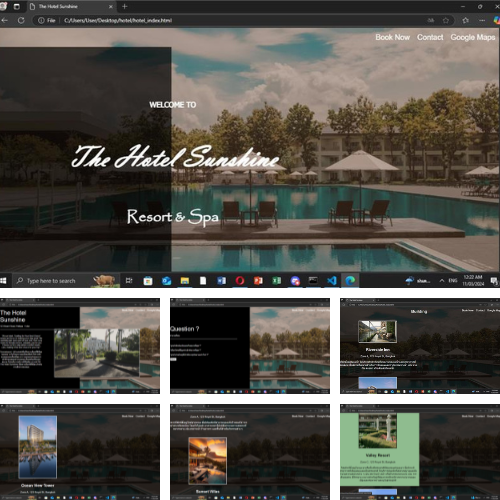
\includegraphics[scale=0.50]{page1.png}
\caption{หน้าเว็บไซต์} 
\label{fig:graph16}
\end{figure} 

\begin{figure}[h!]
\centering
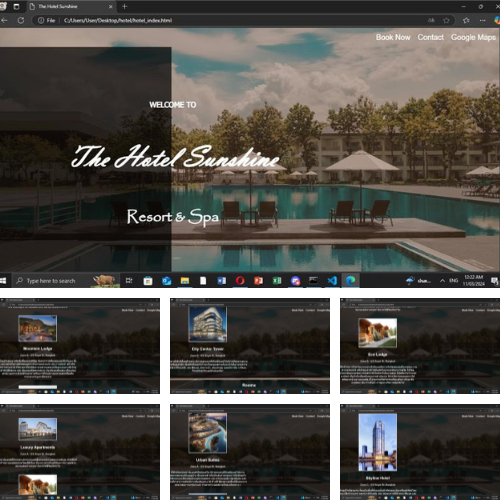
\includegraphics[scale=0.50]{page2.png}
\caption{หน้าเว็บไซต์} 
\label{fig:graph17}
\end{figure} 

\begin{figure}[h!]
\centering
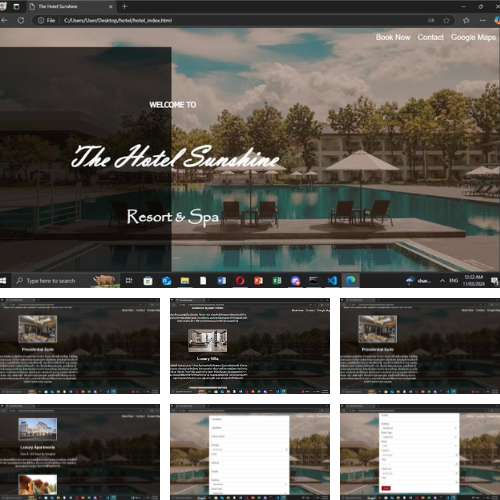
\includegraphics[scale=0.50]{page3.png}
\caption{หน้าเว็บไซต์} 
\label{fig:graph18}
\end{figure} 

\chapter{บทสรุป}
การสร้างระบบฐานข้อมูลและการพัฒนาเว็บเพจร่วมกันนั้น สามารถตอบสนองความต้องการของผู้ที่สนใจได้ โดยต้องอาศัยความเข้าใจทั้งการออกแบบโครงสร้างข้อมูลและการสร้างส่วนติดต่อผู้ใช้ที่ใช้งานง่าย รวมถึงการทดสอบและการบำรุงรักษาระบบเพื่อให้ใช้งานได้อย่างมีประสิทธิภาพและปลอดภัยตลอดเวลา


\printbibliography
\end{document}
 

 